\documentclass[../main.text]{report}
\begin{document}
\subsection{Première conjecture}
\subsubsection{Introduction}

La conjoncture que nous allons tester ici est la suivante: 
Pour tout $n = 6, 7, ...$, il existe un nombre premier $p$ tel que $6n-p$ et $6n+p$ sont tous les deux premiers. \footnote{Conjecture 2.3 de ...}

Nous allons d'abord vérifier que cette conjecture tient pour les nombres premiers, puis vérifier si celle-ci tient aussi pour les ensembles aléatoires suivant leur distribution.
La procédure pour analyser cette conjecture est donc la suivante: pour chaque $n\in \mathbb{N}, 6 \leq n \leq 10000$, nous vérifierons si l'assertion tient. Nous collecterons alors tout $n$ tel que $\neg P(n)$ dans un tableau de données afin d'analyser, pour chaque ensemble ou chaque groupe d'ensemble, le nombre et la distribution des erreurs.

%Nous utiliserons ici les ensembles générés précedemment, ainsi que plusieurs ensembles contrôles. 
%Ces ensembles contrôles possèdent les mêmes cardinaux que 

\subsubsection{Analyse}


%Utilisons les notations $R_{k_n}$, $U_{k_n}$ pour désigner les ensembles $\{i \in R_k ~|~i < n \}$ (respectivement, $\{i \in R_k ~|~i < n \}$).
Soit $P(n)$ l'assertion "Il existe $p \in R_{k_n}, p \geq 6$ tel que $6n-p \in R_k$ et $6n+p \in R_k$".

En utilisant un algorithme \footnote{voir /py\_code/... }, nous avons pu observer que l'assertion est vraie pour tout $n \leq 10^5$.

Le graphique \ref{fig:failures_2_3} ci-dessous représente en abscisses le nombre total d'erreur (c'est à dire le nombre d'entiers $n$ tel que $\neg P(n)$ pour un certain ensemble) et en ordonées le plus grand entier pour laquelle l'assertion est fausse. Chaque point représente un ensemble tel que défini précedemment.

\begin{figure}[H]
\centering
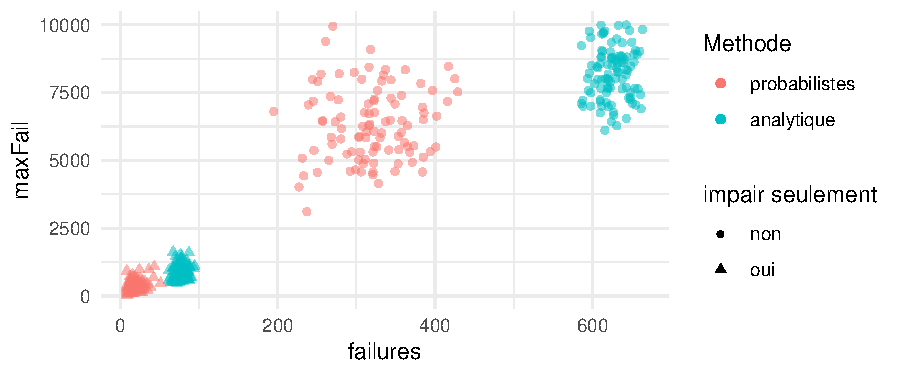
\includegraphics{plot_failure_maxfaile_c_2_3}
\caption{}
\label{fig:failures_2_3}
\end{figure}

Nous debuterons par remarquer que les ensembles non restraints aux nombres impairs génerent un nombre assez conséquent d'erreurs: plus de 200 erreurs pour la quasi-totalité de ces ensembles. 
De plus, ces erreurs persistent assez tardivement: pour la majorité de ces ensembles, il existe (au moins) un entier $n > 5000$ pour lequel l'assertion est fausse.
Cependant, les ensembles composés de nombres impairs ont un nombre relativement faible d'erreurs (moins de 50 pour les ensembles générés par l'algorithme probabilistique, moins de 100 pour les ensembles générés par les algorithmes analytiques, voir figure [x]). 
De plus, le plus grand entier pour lequel l'assertion n'est pas vérifiée est relativement faible: cela signifie que pour tout entier $n > 2500$, l'assertion est vérifiée.  

%\begin{itemize}
	%\item le nombre de success: $S := \#\{n \in \mathbb{N}~|~P(n)\}$,
	%\item le nombre d'echecs: $F := \#\{n \in \mathbb{N}~|~\neg P(n) \}$, 
	%\item le plus grand entier pour lequel l'assertion n'est pas vérifiée: $M := \max\{n \in {N}~|~\neg P(n) \}$
%\end{itemize}

Les diagrammes à boites \ref{fig:boxplots} et \ref{fig:boxplots_Odd} ci-dessus offrent un appercu de la distribution des erreurs

\begin{figure}[H]
\centering
	\subfigure[Plus grand n ne vérifiant pas l'assertion]{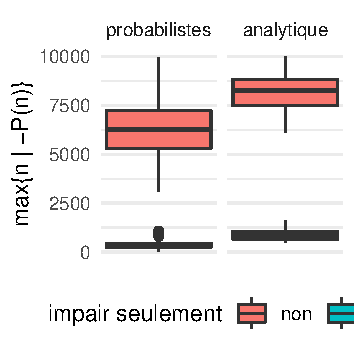
\includegraphics{C23_MaxFail_BoxPlot}}%
	\subfigure[Nombre d'erreurs]{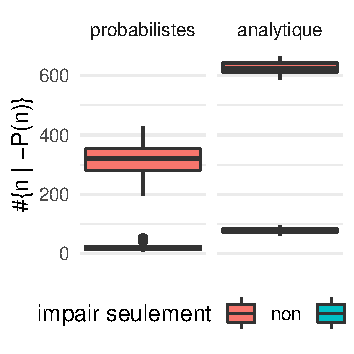
\includegraphics{C23_FailCount_BoxPlot}}
	\caption{Diagrammes en boite}
	\label{fig:boxplots}
\end{figure}

\begin{figure}[H]
\centering
	\subfigure[Plus grand n ne vérifiant pas l'assertion]{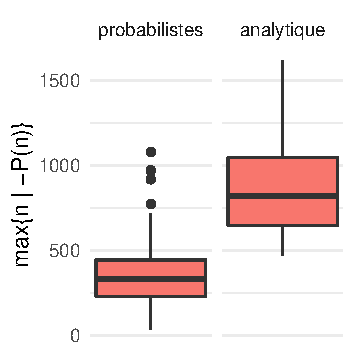
\includegraphics{C23_MaxFail_BoxPlot_Odd}}%
	\subfigure[Nombre d'erreurs]{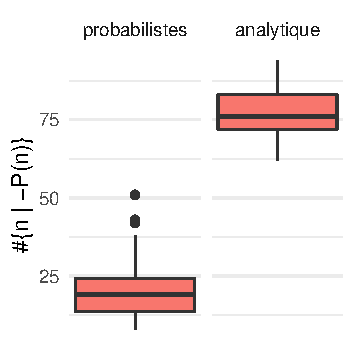
\includegraphics{C23_FailCount_BoxPlot_Odd}}
	\caption{Diagrammes en boite - ensembles impairs.}
	\label{fig:boxplots_Odd}
\end{figure}
Il existe parmis ces ensembles 3 ensembles vérifiant l'assertion pour tout $n, 100 \leq n \leq 10000$:
\begin{itemize}
	\item l'ensemble probabiliste impair 032 dont le plus grand entier ne vérifiant pas l'assertion est 38
	\item l'ensemble probabiliste impair 091 dont le plus grand entier ne vérifiant pas l'assertion est 74
	\item l'ensemble probabiliste impair 033 dont le plus grand entier ne vérifiant pas l'assertion est 97
\end{itemize}

\subsubsection{Conclusion de l'analyse}

\begin{figure}[H]
\centering
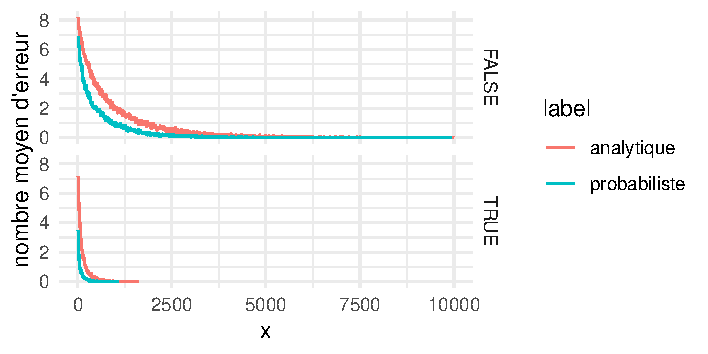
\includegraphics{conjecture_2_3_10k_bin5_line}
\caption{Diagramme représentant le nombre moyen d'erreur (entier ne vérifiant pas P) sur l'interval $(n,n+5]$}
\label{fig:conjecture_2_3_10k_bin5_line}
\end{figure}

\begin{figure}[H]
\centering
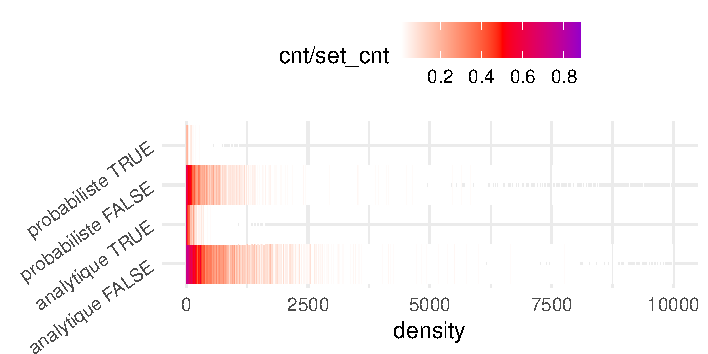
\includegraphics{heat_conjecture_2_3}
\caption{Diagramme représentant le nombre moyen d'erreur (entier ne vérifiant pas la conjecture) sur l'interval $(n,n+5]$}
\label{fig:heat_conjecture_2_3		}
\end{figure}
\end{document}